\section{Situación y relieve de España}

\subsection{Situación de España}

El territorio español se sitúa en el hemisferio norte, concretamente en el suroeste de Europa (Figura \ref{fig:mapa-fisico-europa}). España está formada por gran parte de la península ibérica, el archipiélago de Canarias en el océano Atlántico, el de Baleares en el mar Mediterráneo y las ciudades autónomas de Ceuta y Melilla, en el norte del continente africano.

\vspace{3mm}
La España peninsular limita:

Al norte, con el mar Cantábrico, Francia y Andorra. Al sur, con el océano Atlántico y el mar Mediterráneo. Al este, con el mar Mediterráneo. Al oeste, con el océano Atlántico y Portugal, que también forma parte de la península ibérica. Los archipiélagos balear y canario están bañados por el mar Mediterráneo y el océano Atlántico, respectivamente.

\subsection{Relieve de España}

El relieve de España (Figura \ref{fig:mapa-fisico-españa}) es muy variado y tiene una altitud media elevada (650 metros). Es el segundo país con mayor altitud media en Europa, después de Suiza, debido a las grandes cordilleras y sistemas montañosos, y a una meseta central elevada que ocupa gran parte del territorio peninsular.

\begin{figure}[!ht]
    \centering
    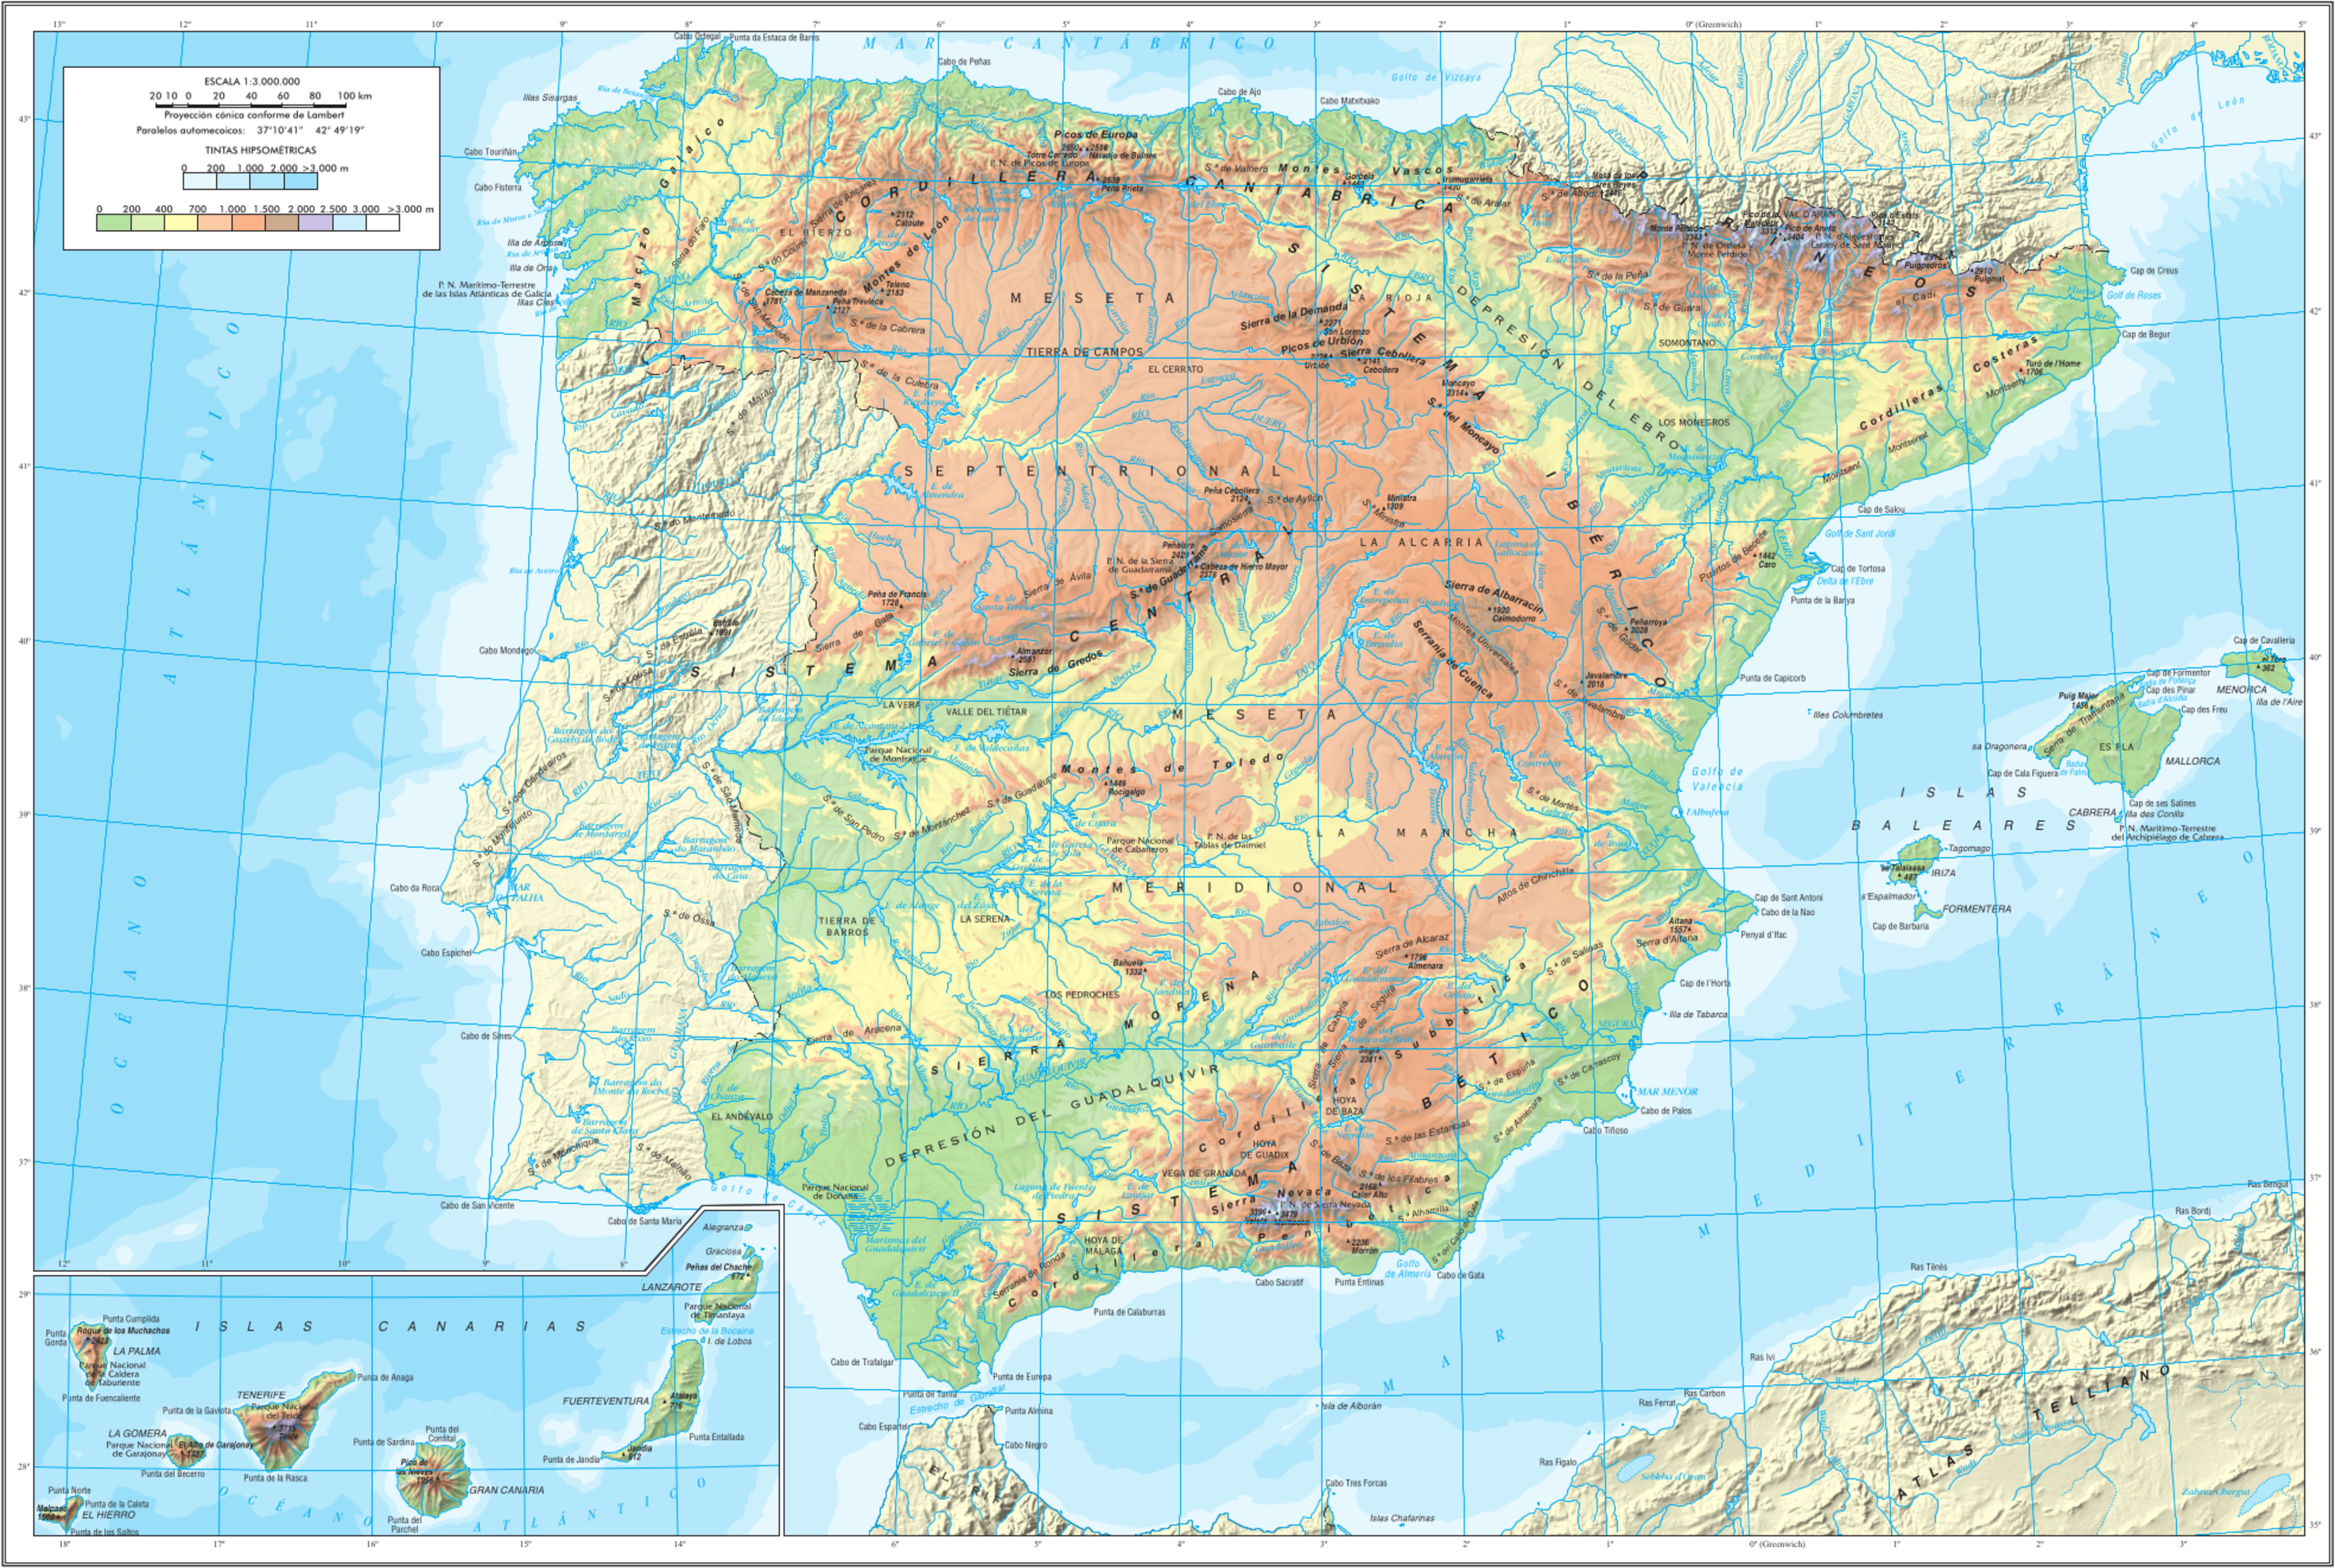
\includegraphics[width=1\linewidth]{Tema2/02_mapa-fisico-espana-normal.pdf}
    \caption{Mapa físico de España}
    \label{fig:mapa-fisico-españa}
\end{figure}

\subsubsection{Relieve de interior peninsular}

Las unidades que forman el relieve peninsular se organizan en torno a una gran meseta central, sistemas montañosos que la bordean y cadenas montañosas y depresiones exteriores a esta.

\vspace{3mm}
\textbf{Meseta}

\vspace{3mm}
La Meseta es una llanura elevada con una altitud media de unos 650 metros. En su interior se sitúan dos sistemas montañosos: el sistema Central y los Montes de Toledo.

\vspace{3mm}
\textbf{Sistema Central}

\vspace{3mm}
Se encuentra en el centro de la Meseta y la divide en dos: \textbf{submeseta norte}, que está ocupada porel valle del río Duero, y la \textbf{submeseta sur}, con los valles de los ríos Tajo y Guadiana. La submeseta norte es más extensa y elevada que la sur. Sus principales sierras son las de Somosierra, Guadarrama, Gata y Gredos, donde se localiza la cima más alta, el pico Almanzor (2 592 m).

\vspace{3mm}
\textbf{Unidades que bordean la Meseta}

\vspace{3mm}
\textbf{Montes de León}

\vspace{3mm}
Se encuentran al noroeste de la Península. Destacan las sierras de Teleno y Segundera, que alcanza los 2 000 m.

\vspace{3mm}
\textbf{Cordillera Cantábrica}

\vspace{3mm}
Se localiza en el norte de la Península, paralela a la costa. Su montaña más alta es Torrecerredo (2 648 m), en los Picos de Europa.

\vspace{3mm}
\textbf{Sistema Ibérico}

\vspace{3mm}
Se sitúa en el este peninsular, entre la Meseta y la depresión del Ebro. Sus principales sierras son Picos de Urbión, sierra de Albarracín y sierra del Moncayo, donde se localiza su pico más alto, el Moncayo (2 313 m).

\vspace{3mm}
\textbf{Sierra Morena}

\vspace{3mm}
Se encuentra en el sur de la Península y separa la Meseta del valle del Guadalquivir. Destacan las sierras de Aracena, de Hornachuelos y Sierra Madrona, donde está la cima más alta, Bañuela (1 323 m).

\subsubsection{Relieve de interior peninsular}

\textbf{Unidades del relieve exteriores a la Meseta}

\vspace{3mm}
\textbf{Macizo Galaico}

\vspace{3mm}
Se encuentra en el extremo noroeste de la Península. Se caracteriza por su poca altitud, relieve poco pronunciado y cumbres redondeadas. Sobresale el pico de Cabeza de Manzaneda (1 778 m), en el centro del macizo.

\vspace{3mm}
\textbf{Montes Vascos}

\vspace{3mm}
Se localizan en el norte, entre la cordillera Cantábrica y los Pirineos. Son un conjunto de montañas no alineadas y de relieve desigual. Uno de sus picos más altos es Aitzkorri (1 528 m).

\vspace{3mm}
\textbf{Pirineos}

\vspace{3mm}
Están situados en el noreste de la Península y se extienden desde el golfo de Bizkaia (mar Cantábrico) hasta el cabo de Creus (mar Mediterráneo). Constituyen una frontera natural entre España, Andorra y Francia. Se caracterizan por la elevada altitud de sus montañas, que alcanzan los 3 000 m. Su pico más alto es el Aneto (3 404 m).

\vspace{3mm}
\textbf{Cordillera Costero-Catalana}

\vspace{3mm}
Se localiza entre los Pirineos y la desembocadura del río Ebro. Forma un paisaje de sierras de poca altura en paralelo a la costa mediterránea. Su pico más alto es el Turó de l’Home (1 712 m).

\vspace{3mm}
\textbf{Cordilleras Béticas}

\vspace{3mm}
Son un gran conjunto montañoso en el sureste peninsular, que se extiende desde el estrecho de Gibraltar hasta el cabo de la Nao, en Alicante. Está formado por dos cordilleras que discurren casi paralelas: la Penibética y la Subbética.

\begin{itemize}
    \item La \textbf{cordillera Penibética} es la que está situada más próxima a la costa y sus montañas son elevadas. En Sierra Nevada se encuentra el pico más alto de la Península, el Mulhacén (3 478 m).
    \item La \textbf{cordillera Subbética} se localiza en el interior, junto al borde sur de la Meseta. Es menos elevada que la Penibética.
\end{itemize}

\textbf{Depresiones exteriores a la Meseta}

\vspace{3mm}
En la Península, entre los bordes de la Meseta y las cordilleras exteriores, se localizan dos grandes depresiones por las que discurren los ríos Ebro y Guadalquivir, de ahí sus nombres.

\vspace{3mm}
\textbf{Depresión del Ebro}

\vspace{3mm}
Es una extensa llanura de forma triangular, encajada entre el sistema Ibérico y los Pirineos. Por ella discurre el río Ebro, en cuya desembocadura deposita los materiales que arrastra a lo largo de su curso, dando lugar a una zona de tierra que entra en el mar, llamada delta.

\vspace{3mm}
\textbf{Depresión del Guadalquivir}

\vspace{3mm}
Es también una llanura triangular, encajada entre Sierra Morena y la cordillera Subbética. La atraviesa el río Guadalquivir, en cuya desembocadura el mar inunda los terrenos bajos y forma marismas, que son zonas muy fértiles.

\subsubsection{El relieve costero peninsular}

España tiene unos 5 970 km de costa repartidos entre el litoral peninsular, los archipiélagos balear y canario, y las ciudades de Ceuta y Melilla. Nuestras costas son, en general, rectas sin muchos entrantes y salientes, exceptuando la costa gallega. Predominan las costas altas y acantiladas, aunque también hay costas bajas con grandes playas.

\vspace{3mm}
\textbf{Costa atlántica}

\vspace{3mm}
Se divide en tres grandes grupos: la cantábrica, la atlántica gallega y la atlántica andaluza.

\vspace{3mm}
La \textbf{costa cantábrica} se extiende desde la desembocadura del río Bidasoa hasta el cabo de Ortegal. Es recta, alta, acantilada y rocosa debido a la proximidad de la cordillera Cantábrica al mar. También hay rías o valles inundados por la entrada de mar en el tramo final de un río y playas. Destacan accidentes del relieve como los cabos de Peña, Ajo y Matxitxaco, y el golfo de Bizkaia.

\vspace{3mm}
La \textbf{costa atlántica gallega} abarca desde el cabo de Ortegal hasta la desembocadura del río Miño. Es alta, rocosa y muy recortada por la existencia de numerosas rías. Sus accidentes más significativos son las rías de Arousa, Vigo y Pontevedra, y el cabo Fisterra.

\vspace{3mm}
La \textbf{costa atlántica andaluza} se localiza desde la desembocadura del río Guadiana, en la frontera con Portugal, hasta el estrecho de Gibraltar. Es recta, baja y arenosa, debido a la cercanía de la depresión del Guadalquivir. En ella hay marismas, dunas y playas largas y arenosas. Se pueden mencionar accidentes, como el golfo de Cádiz.

\vspace{3mm}
\textbf{Costa mediterránea}

\vspace{3mm}
Se divide en dos grupos: la mediterránea del sur y la mediterránea del este. En esta última se distinguen, asimismo, dos tramos: la valenciana y la catalana.

\vspace{3mm}
La \textbf{costa mediterránea del sur} se extiende desde el estrecho de Gibraltar hasta el límite de la Región de Murcia con la Comunidad Valenciana. Es recta, alta y acantilada debido a la cercanía de la cordillera Penibética, que discurre en paralelo a la costa. También presenta algunos tramos llanos en la zona de Málaga. Entre sus accidentes destacan el golfo de Almería y los cabos de Gata y Palos.

\vspace{3mm}
La \textbf{costa mediterránea del este} presenta dos tramos: el de la costa valenciana y el de la costa catalana.

\begin{itemize}
    \item La \textbf{costa valenciana} comprende desde la Vega Baja del Segura hasta el delta del Ebro. Es baja y arenosa con amplias llanuras litorales. También hay algunas zonas altas y rocosas, como el cabo de la Nao.
    \item La \textbf{costa catalana} se extiende desde el delta del Ebro hasta el límite con Francia. Es recortada, alta, acantilada y rocosa. Sus principales accidentes del relieve son el cabo de Creus y el golfo de Roses.
\end{itemize}

\subsubsection{El relieve de los archipiélagos}

Los archipiélagos, además de estar situados en mares diferentes, el de Baleares en el Mediterráneo y el de Canarias en el océano Atlántico, presentan relieves distintos.

\vspace{3mm}
\textbf{El relieve de Baleares} (Figura \ref{fig:relieve-baleares})

\vspace{3mm}
Baleares se localiza en el mar Mediterráneo, frente a la costa oriental de la Península. Su \textbf{relieve} es en general montañoso y está relacionado con el de la Península. En Mallorca, Eivissa y Formentera, el relieve es una prolongación del sistema Bético, y en Menorca, de la cordillera Costero-Catalana. La mayor altitud es el pico de Puig Major (1 445 m), en la sierra de Tramuntana (Mallorca). Las \textbf{costas} son altas y recortadas, especialmente en el norte de Mallorca y de Menorca.

\begin{figure}[!ht]
    \centering
    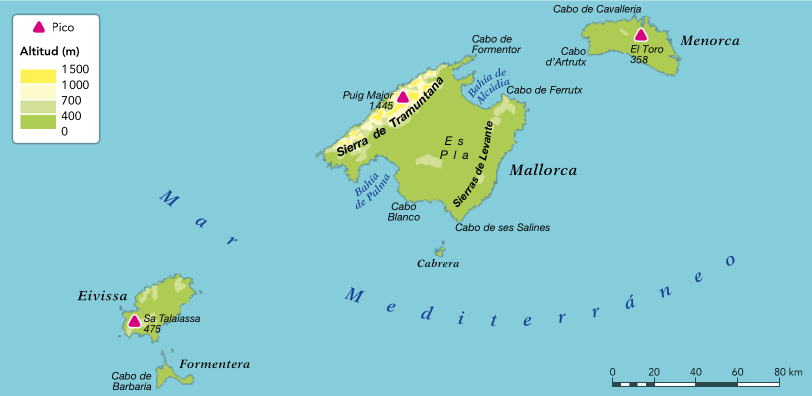
\includegraphics[width=0.7\linewidth]{Tema2/03_relieve_Baleares.png}
    \caption{El relieve de Baleares}
    \label{fig:relieve-baleares}
\end{figure}

\textbf{El relieve de Canarias} (Figura \ref{fig:relieve-canarias})

\vspace{3mm}
Canarias está situada en el océano Atlántico, frente a las costas del norte de África. El \textbf{relieve} es montañoso y de origen volcánico, lo que ha originado un paisaje muy peculiar. El pico más alto de España se encuentra en la isla de Tenerife, el Teide, un volcán de 3 718 m. Las \textbf{costas} son, en general, altas, acantiladas y poco recortadas, aunque en el sur de las islas hay también playas. En las islas occidentales son de cantos, y en las orientales, de arena.

\begin{figure}[!ht]
    \centering
    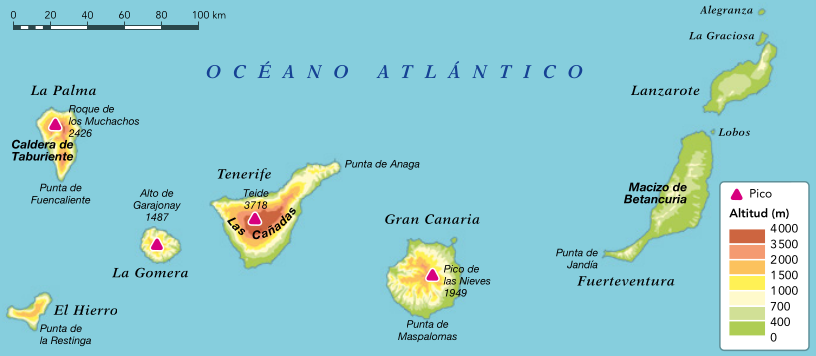
\includegraphics[width=0.7\linewidth]{Tema2/04_relieve_Canarias.png}
    \caption{El relieve de Canarias}
    \label{fig:relieve-canarias}
\end{figure}

\subsubsection{El relieve de Andalucía}

Andalucía (Figura \ref{fig:mapa-fisico-andalucia}) es la comunidad autónoma más extensa de España y la más meridional de la Península. Su relieve es muy variado, la mayor parte de su territorio es llano, pero cuenta con dos grandes zonas montañosas al norte y al sureste.

\vspace{3mm}
\textbf{Las zonas montañosas}

\vspace{3mm}
Las zonas montañosas se extienden por el norte, el sur y el este de Andalucía:

\begin{itemize}
    \item \textbf{Sierra Morena} ocupa la zona norte y forma el borde sur de la Meseta. Sus sierras, perpendiculares al Guadalquivir, presentan alturas moderadas.
    \item Las \textbf{cordilleras Béticas} se extienden por el sur y el este, y están formadas por dos cordilleras:
    \begin{itemize}
        \item La \textbf{Subbética}, al norte, es la menos elevada de las dos. Su máxima altura es el pico de La Sagra (2 381 metros).
        \item La \textbf{Penibética}, al sur, discurre paralela a la costa mediterránea y es más elevada. El pico Mulhacén, en Sierra Nevada, es el de mayor altura de Andalucía (3 479 metros).
    \end{itemize}
\end{itemize}

\begin{figure}[!ht]
    \centering
    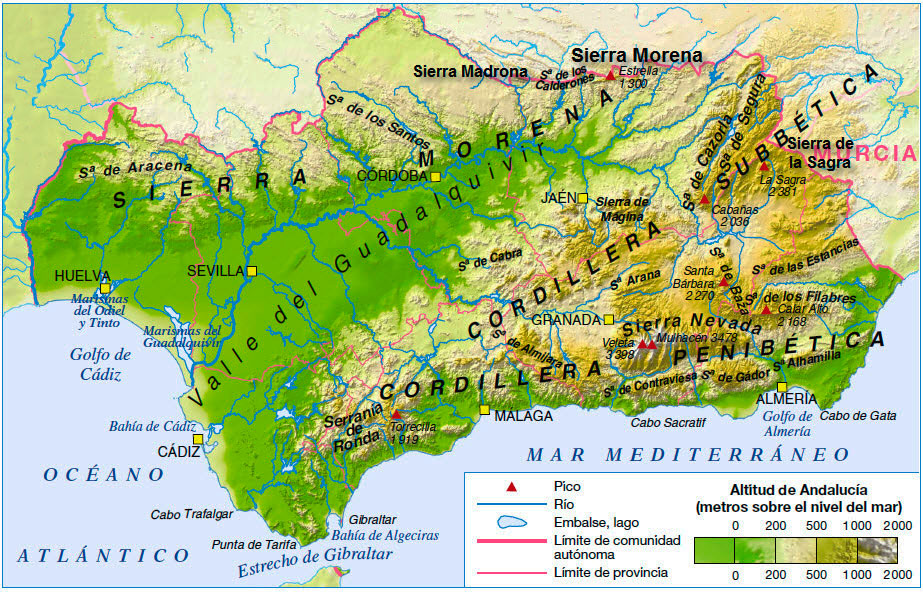
\includegraphics[width=0.7\linewidth]{Tema2/05_mapa-fisico-andalucia.jpg}
    \caption{Mapa físico de Andalucía}
    \label{fig:mapa-fisico-andalucia}
\end{figure}

\textbf{El valle del Guadalquivir}

\vspace{3mm}
Se extiende entre Sierra Morena y el sistema Bético. Es una \textbf{gran llanura de tierras bajas y fértiles}, y de forma triangular. Su altitud media, de 100 metros sobre el nivel del mar, hace de ella una de las zonas más bajas de la Península. Por todo el valle se extienden llanuras fértiles llamadas \textbf{campiñas}. Las \textbf{vegas} son los terrenos agrícolas situados a la orilla de los ríos.

\vspace{3mm}
\textbf{Las costas andaluzas}

\vspace{3mm}
En Andalucía distinguimos dos zonas costeras, la atlántica y la mediterránea, a un lado y a otro del estrecho de Gibraltar. La \textbf{costa atlántica} corresponde por completo con las zonas llanas del valle del Guadalquivir. Por tanto, es una costa baja y arenosa, con grandes playas donde se forman dunas, como en las costas de Cádiz y de Huelva. En la desembocadura de los ríos, el mar invade las zonas más bajas cuando hay marea alta, formando marismas.

\vspace{3mm}
La \textbf{costa mediterránea} está condicionada por la proximidad de la cordillera Penibética. Por tanto, es predominantemente recta, alta y acantilada, aunque presenta algunas zonas más llanas, como en la costa de Málaga.